%!TEX root = ../report.tex

\documentclass[../report.tex]{subfiles}
\begin{document}

\subsection{Context}

To better understand the relevance of the following literature review, we first provide a brief overview of where the concepts to follow fit into our work so far. We will begin by discussing The Firefighter Problem and explain how it can be adapted to a rudimentary model of disease. A huge amount of our research (in particular, the more experimental strand) has started with this problem as its foundation and in the following section we will explain the ways we have extended the classic problem in stochastic and game-theoretic directions. Hence, we believe a detailed discussion into the classic problem and some key results thereof as crucial to understanding our work so far.

We then move on to discuss compartmental graph models of disease, in particular examining the differential equations required to describe such models exactly. This has formed the basis of our more formal work over the past year, so again a discussion of the results and knowledge in this field that pre-dates our work provides important background to the work we have done. While this work appears fairly distinct in character to the more experimental prong of our approach, the two aspects are related in principle. That is, both directions aim to take existing approaches to disease modelling and introduce a new way of representing protection from disease, both as an external defence strategy and as an internal inclination in individuals, here represented by adding a new compartment to existing compartmental models.

We end this section with a discussion of Percolation Theory and its use in a graph-theoretic context. We have identified this as an important tool for disease modelling using graphs but we have not yet employed it to a significant extent. We will, nonetheless, discuss the areas that we believe it would prove most useful in the following section on the work completed so far. While percolation theory has yet to find itself in a significant way into our work, we expect that it could be useful in either (or both) of the two main aspects, but more so in the experimental prong of our approach. Specifically, we expect to use percolation in modelling more interesting stochastic fire propagation as well as generating randomly percolated graphs on which to play the game. 

\subsection{The Firefighter Problem}

The Firefighter Problem, which we refer to as simply {\scshape Firefighter}, was first introduced by Hartnell \cite{hartnell_1995} and models an outbreak of fire with a firefighter strategically blocking its path. {\scshape Firefighter} has been the primary foundation for our approaches to modelling over the last year.

We formalise {\scshape Firefighter} as follows: at $t=0$, a fire breaks out at some vertex $v_0$ of graph $G$. The firefighter then `protects' another vertex\footnote{\,This has been extended to $n$ vertices in some research, but here we wish to illustrate for simplicity the original single-vertex outbreak form of the problem.} of $G$. A protected vertex is protected for the remainder of the game; it is inflammable \textit{ad infinitum.} Similarly, a vertex that has been on fire is `burnt' for the rest of the game and cannot ignite again. The fire spreads to any immediate neighbouring vertices that are neither protected nor burnt. Then, the firefighter may protect another vertex, the fire spreads again and so on. The following is a decision formulation given by Finbow and MacGillivray for {\scshape Firefighter} \cite{finbow_2009}:
\vspace{1mm}

\begin{center}
\noindent\fbox{%
	\centering\parbox{0.8\linewidth}{%
{\scshape Firefighter}\\ \indent
{\scshape Instance:} A rooted graph $(G,r)$ and an integer $k\geq 1$.\\ \indent
{\scshape Question:} Is there a finite sequence $d_1, d_2,\dots d_t$ of vertices of the graph $G$ such that:
	\begin{enumerate}[label=\roman*]
		\item $d_i$ {is neither burned nor defended at time} $i$,
		\item {At time} $t$, no undefended vertex is adjacent to a burning vertex, and
		\item {At least} $k$ {vertices are saved at the end of time} $t$?
	\end{enumerate}
	}%
}%
\end{center}

Common problems in classic {\scshape Firefighter} often involve how to minimise the number of vertices that will be burnt and, in a given class of trees, determining the average number of burnt vertices. There are several results available to us in classic {\scshape Firefighter}. For one, the problem is NP-complete even if restricted only to trees with maximum degree three. Further, the problem is solvable in polynomial time for graphs of maximum degree three, so long as the fire starts at a vertex of degree two \cite{finbow_2009}. We also have some results regarding game strategies, such as that the greedy algorithm is a $1/2$-approximation for the problem on trees \cite{finbow_2009}.

If we let each vertex be an individual and let the edges between them represent social contact. This is a simple model for disease infection, which is where our interest in the game enters. There are many natural contextualisations of {\scshape Firefighter} beyond modelling disease spread, which we may choose to apply our work to in future - for instance, we may think of edges representing virtual contact between individuals on social media, yielding a model for the spread of viral internet memes \cite{obrien_2019}.

%%%%%%%%%%

\subsection{Markovian SIR epidemics on networks}
\label{subsec:SIR-lit}

Compartmental models are mathematical ways of simulating how compartments of a population interact. This involves systems of equations describing the behaviour of each compartment and then seeing how each compartment interacts with the others. These compartments can describe many states an individual (typically a person or an animal) can be in - for instance, we could use predator/prey compartments to simulate a hunting situation or susceptible/infected/recovered compartments to model disease spread. In this discussion, we will begin by discussing the standard $SIR$ model, explain how it can be extended to a graph-theoretic context and then - crucially, for understanding our work so far - explain the current work on generating a system of equations to exactly describe such a model.

\subsubsection{Standard $SIR$ model with fixed population}

The SIR Model is a compartmental epidemiological model with three compartments (generally referred to as `states') related to an epidemic: {\it susceptible, infected} and {\it recovered.} We define $S(t)$ as the number of people who do not currently have but are able to contract the infection at time $t$, $I(t)$ as individuals who currently have the disease and are infectious and finally $R(t)$ as those who have had the disease and subsequently recovered, granting them at least some level of immunity in certain contexts. For a fixed population $N$, we have that $S(t) + I(t) + R(t) = N$ - that is, we assume a fixed population where we do not wish to consider vital dynamics, usually when an epidemic is short-lived. Then, for $\beta$ and $\gamma$ the rates of infection and recovery respectively, the standard SIR model without vital dynamics (birth and death rates) is given as follows:

\begin{align}
\frac{dS}{dt} & = -\beta \frac{SI}{N} \label{dS}\\
\frac{dI}{dt} & = \beta\frac{SI}{N} \gamma I \label{dI}\\
\frac{dR}{dt} & = \gamma I - \mu R \label{dR}
\end{align}

We generally aren't much interested in the expression for $\dot{\langle R \rangle}$, since we require that $ \dot{\langle S \rangle} + \dot{\langle I \rangle} + \dot{\langle R \rangle} = 1$ meaning we can always find the third probability as the compliment of the sum of the other two probabilities. In much of the literature, the convention is for this reason to only give the first two equations.

\subsubsection{Extending the $SIR$ model to graphs}

In order to extend our SIR model to network graphs, we first examine the probability of an agent being in a given class: let $\langle A_i \rangle$ represent the time-independent probability of person $i$ being in state $A$, meaning that the expression of the form $\langle A_i B_i \rangle$ represents the (again, time-independent) probability of individuals $i$ and $j$ being in states $A$ and $B$ respectively \cite{kiss_2014}. We begin with a contact network, where vertices represent individuals and the edges between them represent social contact which may serve as an infection pathway. Then, the adjacency matrix $G$ of this network is constructed by assigning $G_{ij} = 1$ when $i$ and $j$ share an edge and $G_{ij} = 0$ otherwise.\footnote{Because we are infrequently interested in self-transmission, we often set $G_{ii}=0.$} Then, we extend this contact network to a transmission network: let $\beta_i$ represent the per-link infection rate for individual $i$ and $\gamma_i$ represent the recovery rate for $i$. For the transmission matrix $T,$ we assign $T_{ij}=\beta_i$ if there is a route of infection between $i$ and $j$ and $T_{ij}=0$ otherwise. Often, we will consider unweighted and undirected graphs, but in general $T_{ij}$ may not equal $T_{ji}$.\\
We now note that we can replace $\beta_i$ with a term involving such a transmission matrix of a network in order to begin extending the usual SIR model into a network realm. Using the substitution $ \beta_i \frac{SI}{N} = \sum^{N}_{j=1}T_{ij} \langle S_i I_j \rangle,$ the equations become
\begin{align*}
\dot{\langle S_i \rangle} & = -\sum^{N}_{j=1}T_{ij} \langle S_i I_j \rangle\\
\dot{\langle I_i \rangle} & =\sum^{N}_{j=1}T_{ij}\langle S_i I_j \rangle - \gamma_i \langle I \rangle \\
\dot{\langle R_i \rangle} & = \gamma_i \langle I \rangle,
\end{align*}
which are the evolution equations given in \cite{kiss_2014}.

In the past year, we have also spent significant time understanding, applying and expanding results around equations describing Markovian $SIR$ graph models of disease exactly \cite{kiss_2014} so we will now provide a review of the key work in this area and its utility. We will go on to detail the work done so far in extending the results from this paper in the following section.

In \cite{kiss_2014}, the authors note that there are generally three approaches to compartmental models of disease. We can:
\begin{enumerate}
	\item Take averages at population level, 
	\item Maintain a probabilistic view by considering the full state space, or
	\item Begin modelling at the level of vertices and build up to larger structures from there.
\end{enumerate}

The second of the three approaches has been the focus of much of our work, as will be seen in the following section. The latter of these three approaches is the one used in the work on Markovian SIR graph epidemics being discussed currently: begin by considering equations for single vertices, then consider dependencies on pairs, then triples and so on until we reach the full system size. Such equations are well defined and consistent, which is not difficult to see.

The work presented has two aims. Firstly, to provide an exact, deterministic representations of Markovian $SIR$ epidemics on graphs with and without loops. Secondly, to identify a link between the structural properties of the graphs and the viability of closures that can be used to write down exact systems of equations that can be numerically evaluated. In particular, the authors show this structural link is founded on cut-vertices and bridges. Cut-vertices are vertices that, if removed from a connected graph, result in the formation of two (or more) disconnected sub-graphs. Bridges are edges that lie between two cut-vertices.

The authors spend significant time expanding intuitions on the identification of closures, which allow us to approximate or even exactly specify higher-order moments in terms of lower-order moments. They claim this is well known to be feasible for tree-like graphs and for graphs with loops starting from some specific initial conditions. They present some examples to develop the intuition that ``loops cannot be closed by breaking them down to their component parts."

The main result of the work reveals an important relation between structure of the graph used in the epidemic model and types of closures that are feasible using cut-vertices and bridges.

They also prove an impressively general result: if a graph with $N$ vertices and  $E$ edges has $T$ triangles and no larger loops than size 3 (meaning also that triangles cannot have overlapping edges), an upper bound on the size of the system of equations describing the system dynamics can be calculated:
$$
2N + 3E + 7T \leq 10N
$$

The authors also provide a ``recipe-like" approach to establish the feasibility of writing down an exact representation for a given graph even more generally. They use this to provide an upper bound for the number of equations required to describe epidemic dynamics exactly:
$$
\displaystyle N_{EQ}(G)=\sum^P_{i=1}m_if_i - 2\sum^{L}_{j=1}(\text{Ind}(v_{i_j})-1).
$$
where $P$ is the number of distinct sub-graphs produced when the original graph is spliced into independent sub-graphs through cut-vertices, $m_i$ represents the number of equations required to describe the corresponding sub-graph $i$, $f_i$ is the frequency or count of the sub-graph $G_i$ and $\text{Ind}(v_{i_j})$ is the number of sub-graphs to which the cut-vertex $v_{i_j}$ belongs.

This takes a sum across the number of equations for all sub-graphs and adjusts to account for unnecessary multiplications caused by cut-vertices being part of multiple sub-graphs, which is a move made in illustrative examples throughout the work.

%%%%%%%%%%

\subsection{Percolation Theory}
\label{sec:perc}

Widely known and used in physics, statistics and mathematics, Percolation theory involves modelling scenarios as $n$-dimensional graphs, so application to {\scshape Firefighter} is not entirely unexpected. Hence, we will now examine percolation theory in order to later explain the utility we have found it may yield in extending and expanding modelling work from {\scshape Firefighter}.

In percolation, the edges between vertices in the graph can be either `open' or `closed' with probability $p$ and $1-p$ respectively. We can think of percolation problems as liquid being poured onto a porous material and whether there is a path from hole to hole along open paths through the material. Note that removing more and more edges moves us towards a critical point at which removing further edges would cause the graph to fall apart into smaller clusters of vertices and edges that have no access to each other \cite{grimmett_1999}. This is known as `bond' percolation, as edges correspond to bonds in many of its applications.
%\begin{figure}[ht]
%	\centering
%		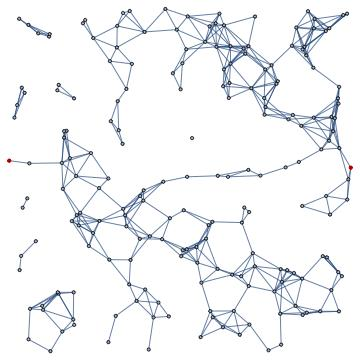
\includegraphics[width=0.45\linewidth]{percolated-graph.jpg}
%	\caption{A graph that has been subject to percolation.}
%	\label{fig:percolated-graph}
%\end{figure}

Several authors have suggested percolation as a possible approach to {\scshape Firefighter} \cite{finbow_2009}. In this context, we could determine the critical point to see how we might contain the fire to a smaller cluster that cannot spread to the wider graph. For {\scshape Firefighter}, site percolation is more applicable: rather than considering open or closed \emph{edges} (`bonds') between vertices as in bond percolation, we consider each \emph{vertex} (`site') as being `occupied' or `unoccupied' with probability $p$ and $1-p$ respectively.

Formally, we consider a point lattice $\mathbb{L}$ and denote the open cluster as $C(x)\text{,~where~}x\in\mathbb{L}$ is the local origin of the cluster. This cluster $C(x)$ is defined as the set of all vertices that can be reached from open paths beginning at the nucleation site, $x$. Then, we are particularly interested in the \emph{percolation probability}:
$$
\theta(p) = \mathbb{P}_p(\,|C(0)|=\infty\,),
$$
and the \emph{critical probability} (or \emph{percolation threshold}):
$$
p_c = \sup\{\,p \mid \theta(p)=0\,\}.
$$
Here, $\mathbb{P}_p$ is the product measure given by:
$$
\displaystyle \mathbb{P}_p=\prod_{v\in\mathbb{L}^d}\mu_v
$$
where $\mu_v$ is the \emph{Bernoulli measure}, which returns $p$ when $v$ is open and $1-p$ when $v$ is closed \cite[p. 28]{klenke_2014}. Analytically, others have shown that in the case of a two-dimensional regular point lattice, the critical probability is $p_c=1/2$ \cite{kersten_1980}.

\end{document}